We conduct experiemnts on the following datasets:

\begin{center}
\begin{tabular}{| l | c |}
  \hline                        
  Dataset Name & Advogato  \\ \hline
  Largest connected component & 5054  \\ \hline
  Size & 6551 vertices  \\ \hline
  Volume & 51332 eges \\ \hline
\end{tabular}
\end{center}

In phase 1, we explored Task 1-3, and do several visualization for experiment results. Figure \ref{fig:results}(a) shows the in degree destribution, we took log of rank to emphasize the effect. Figure \ref{fig:results}(b) shows the out degree destribution, also took logarithm. Figure \ref{fig:pagerank} plots the distribution of different rank value.

\begin{figure}[htbf]
\begin{center}
\begin{tabular}{cc}
     % uncomment the next lines, and give the right ps files
     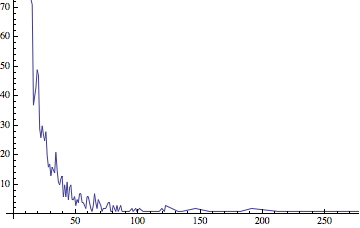
\includegraphics[width=0.4\textwidth]{FIG/indegree.png} &
     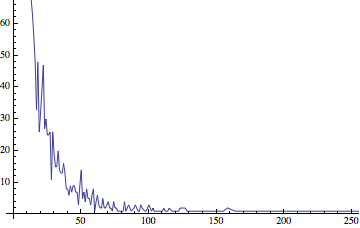
\includegraphics[width=0.4\textwidth]{FIG/outdegree.png} \\
     %\psfig{figure=FIG/plot.ps,width=2in} \\
     % \psfig{figure=FIG/data.ps,width=2in} &
     % \psfig{figure=FIG/plot.ps,width=2in} \\
    (a) & (b) 
\end{tabular}
\caption{In degree distribution (a) and out degree distribution (b)}
\label{fig:results}
\end{center}
\end{figure}

\begin{figure}[htbf]
\begin{center}
     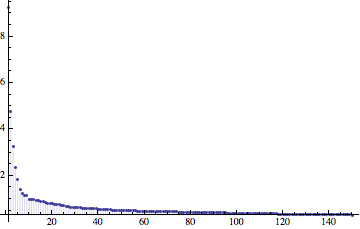
\includegraphics[width=0.6\textwidth]{FIG/pagerank.png}
\caption{Pagerank distribution}
\label{fig:pagerank}
\end{center}
\end{figure}

We also calculated statistics about the weakly connected components as follows.

\begin{center}
\begin{tabular}{| l | c |}
  \hline                        
  Size of WCC & Count  \\ \hline
  1 & 1384  \\ \hline
  2 & 55  \\ \hline
  3 & 1 \\ \hline
  5054 & 1 \\ \hline  
\end{tabular}
\end{center}

